\chapter{Images}
\label{images}

\begin{figure}
    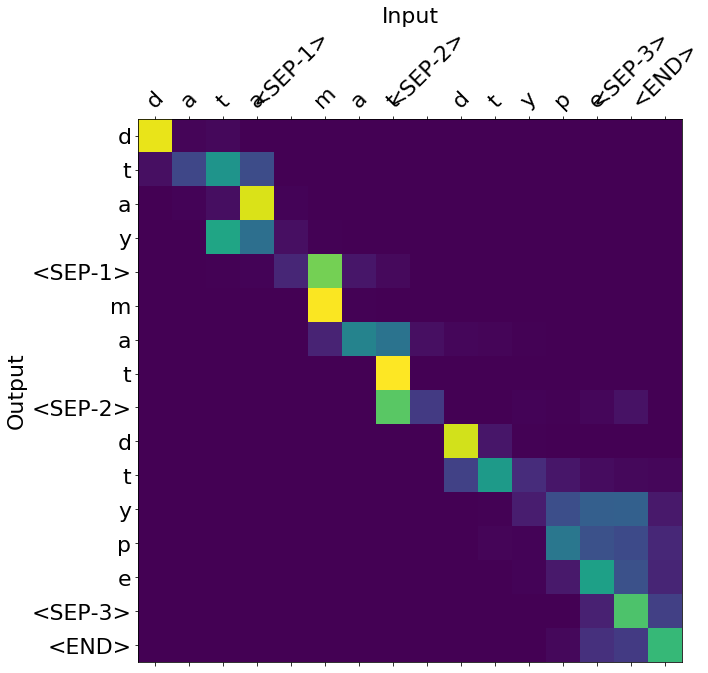
\includegraphics[width=0.8\linewidth]{images/typical_attention.png}
\end{figure}

\begin{table}
\begin{center}
\begin{tabular}{ | c || c |}
    \hline
    \hline
    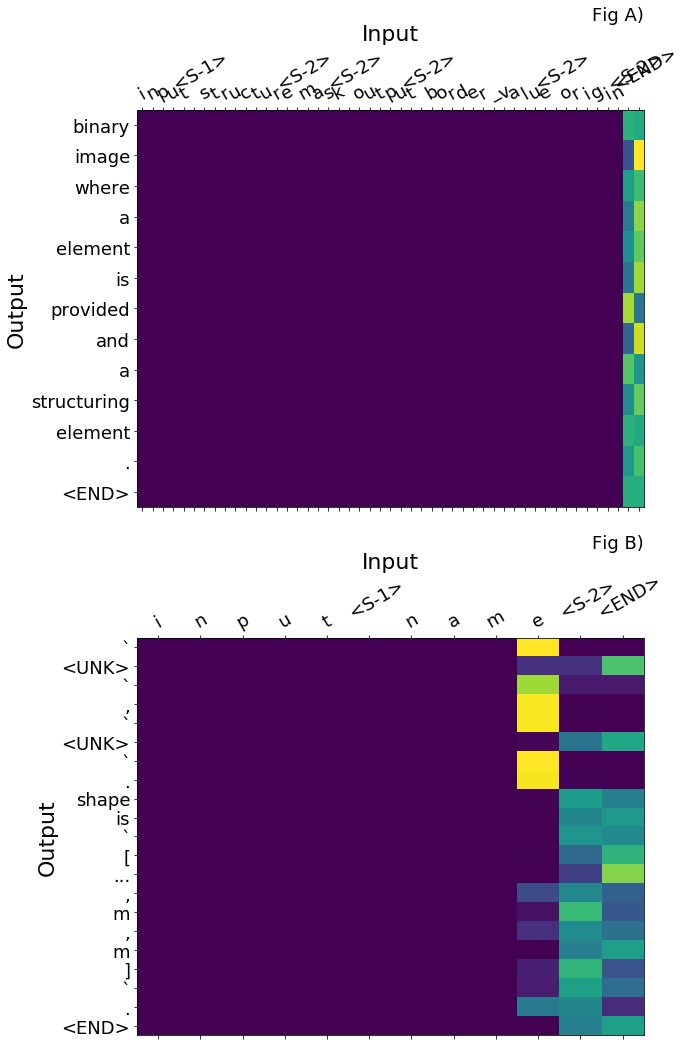
\includegraphics[width=0.5\linewidth]{images/otherargs_example.png}
    &
    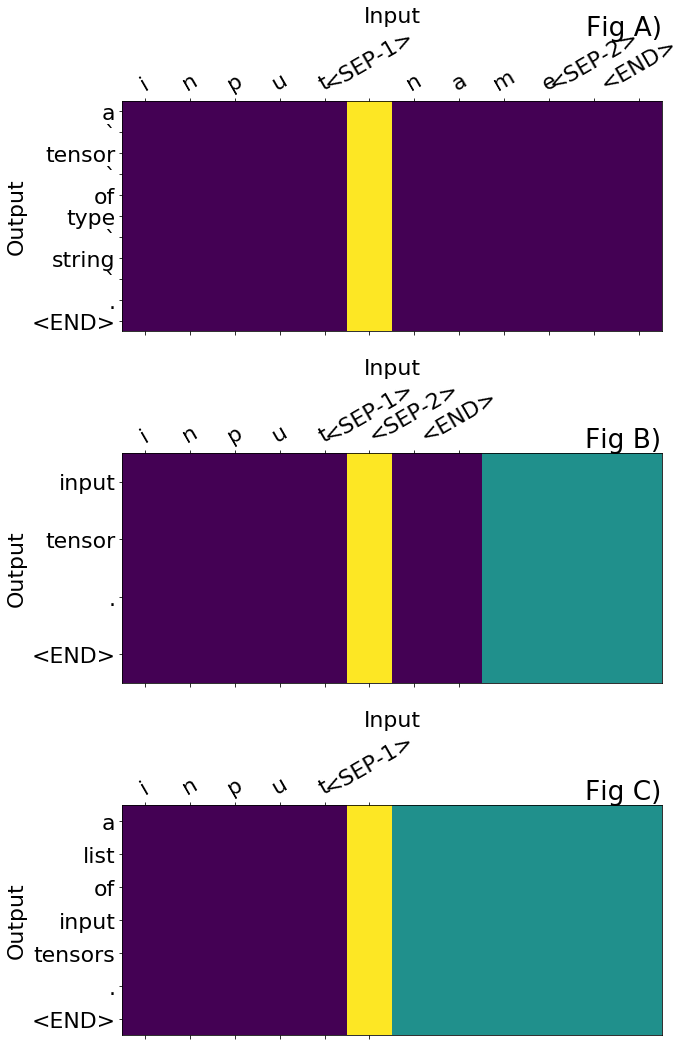
\includegraphics[width=0.5\linewidth]{images/different_translations_dupsXotherargs_3230minib.png} \\


    \hline

    \hline
\end{tabular}
\end{center}
\end{table}



\begin{table}
\begin{center}
\begin{tabular}{ l  }

\textbf{Nonsense}\\

\textbf{I}: \mintinline[]{python}{i n p u t <SEP-1> s t r u c t u r e <SEP-2> m a s k <SEP-2> o u t p}...\\
...\mintinline[]{python}{u t <SEP-2> b o r d e r _ v a l u e <SEP-2> o r i g i n <SEP-2> <END>}\\
\textbf{D}: binary image to be propagated inside ` mask ` .\\
\textbf{P}: binary image where a element is provided and a structuring element . $<$END$>$\\
\\\hline\\


\textbf{Overfitting}\\

\textbf{I}: \mintinline[]{python}{e n c o d i n g _ t y p e <SEP-1> s e l f <SEP-2> d o c u m e}...\\
...\mintinline[]{python}{n t <SEP-2> r e t r y <SEP-2> t i m e o u t <SEP-2> <END>}\\
\textbf{D}: the encoding type used by the api to calculate offsets .\\
\textbf{P}: the encoding type used by the api to calculate sentence offsets . \\
\\\hline\\




\textbf{Underdetermination}\\

\textbf{I}: \mintinline[]{python}{i n p u t <SEP-1> n a m e <SEP-2> <END>}\\
\textbf{D}: a ` tensor ` of type ` complex64 ` . a complex64 tensor .\\
\textbf{P}: ` $<$UNK$>$ ` , ` $<$UNK$>$ ` . shape is ` [ ... , m , m ] ` . \\
\\\hline\\

\\

\end{tabular}

\caption{Three examples of typical errors in the character Seq-to-Seq model.  In this case, the first example shows good use of data in the sequence but is nonsensical. The second is an example of overfitting where the predicted sentence is found in the dataset. The final case, multiple sequences such as these are found in the dataset, each with a different discription. Without looking at code, or function name (in this case) it is impossible to disambiguate and the model fails to make sense }
\end{center}
\end{table}

\begin{table}
\begin{center}
\begin{tabular}{l}

\hline
\textbf{Validation Example}\\

\textbf{I}: \mintinline[]{python}{i n p u t <SEP-1> s t r u c t u r e <SEP-2> m a s k <SEP-2> o u t p}...\\
...\mintinline[]{python}{u t <SEP-2> b o r d e r _ v a l u e <SEP-2> o r i g i n <SEP-2> <END>}\\
\textbf{D}: binary image to be propagated inside ` mask ` .\\
\textbf{P}: binary image where a element is provided and a structuring element . $<$END$>$\\
\\\hline\\

\textbf{Training Examples} starting \mintinline[]{yaml}{i n p u t <SEP-1> s t r u c t u r e}\\
\textbf{I}: \mintinline[]{yaml}{i n p u t <SEP-1> s t r u c t u r e 1 <SEP-2> s t r u c t u r}...\\
...\mintinline[]{yaml}{e 2 <SEP-2> o u t p u t <SEP-2> o r i g i n 1 <SEP-2> o r i g i n 2 <SEP-2> <END>}\\
\textbf{D}: binary image where a pattern is to be detected .\\
\\
\textbf{I}: \mintinline[]{yaml}{i n p u t <SEP-1> s t r u c t u r e <SEP-2> i t e r a t i o n s <SEP-2> o u t }...\\
...\mintinline[]{yaml}{p u t <SEP-2> o r i g i n <SEP-2> m a s k <SEP-2> b o r d e r _ v a l u e }\\
...\mintinline[]{yaml}{<SEP-2> b r u t e _ f o r c e <SEP-2> <END>}\\
\textbf{D}: binary array\_like to be closed . non-zero ( true ) elements form the subset to be closed .\\
\\
\textbf{I}: \mintinline[]{yaml}{i n p u t <SEP-1> s t r u c t u r e <SEP-2> o u t p u t <SEP-2> o r}...\\
...\mintinline[]{yaml}{i g i n <SEP-2> <END>}\\
\textbf{D}: n-dimensional binary array with holes to be filled\\
\\
\textbf{I}: \mintinline[]{yaml}{i n p u t <SEP-1> s t r u c t u r e <SEP-2> o u t p u t <SEP-2> <END>}\\
\textbf{D}: an array-like object to be labeled . any non-zero values in ` input ` are counted as features...\\
...and zero values are considered the background .\\
\\
\textbf{I}: \mintinline[]{yaml}{i n p u t <SEP-1> s t r u c t u r e <SEP-2> i t e r a t i o n s <SEP-2> m a s k }...\\
...\mintinline[]{yaml}{<SEP-2> o u t p u t <SEP-2> b o r d e r _ v a l u e <SEP-2> o r i g i n <SEP-2>}\\
...\mintinline[]{yaml}{b r u t e _ f o r c e <SEP-2> <END>}\\
\textbf{D}: binary image to be eroded . non-zero ( true ) elements form the subset to be eroded .\\
\\
\textbf{I}: \mintinline[]{yaml}{i n p u t <SEP-1> s t r u c t u r e <SEP-2> i t e r a t i o n s <SEP-2> m a s k}...\\
...\mintinline[]{yaml}{<SEP-2> o u t p u t <SEP-2> b o r d e r _ v a l u e <SEP-2> o r i g i n <SEP-2>}\\
...\mintinline[]{yaml}{b r u t e _ f o r c e <SEP-2> <END>}\\
\textbf{D}: binary array\_like to be dilated . non-zero ( true ) elements form the subset to be dilated .\\
\\



\end{tabular}

\caption{A validation example and the a selection of training points. Despite being a long sequence, }
\end{center}
\end{table}

\begin{enumerate}
    \item The rnn final state acts as a good contextual vector for generation, we get good performance improvements on decoding
    \item However, the attention is being pathological. It's such a good strategy, that it stays there, and stops looking elsewhere, the weight decays to zero
    \item then when you get to genuinely hard points - where attention is useful, it cant learn and it panics (see bluring at end - can only explore nearest by states)/
    \item this pattern is noticeable in other locations, moving the lstm to more data (with duplicates), we learn that the lstm learns
    \item this happens even early in training and even with smaller lstm size, and larger datasets too
\end{enumerate}


\begingroup
\begin{table}
\begin{center}
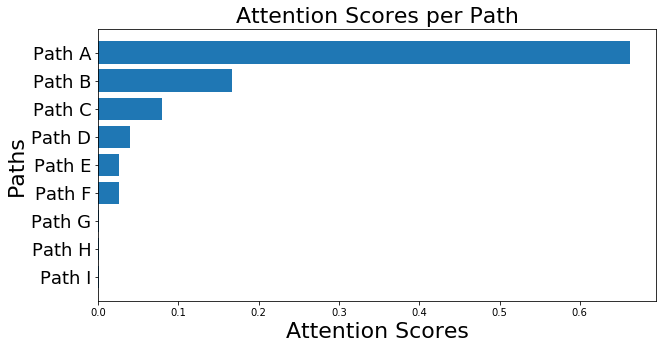
\includegraphics[width=0.8\linewidth]{ImagesCodeRelated/attention_xkcd.png}
    \fontsize{10pt}{12pt}\selectfont
        % how to set font size here to 10 px ?  
\begin{tabular}{c l}
    & \textbf{Paths} \\
    \\
    \textbf{Path A} & Name $\leftarrow$ comprehension $\leftarrow$ ListComp $\leftarrow$ Assign $\rightarrow$ Name : \mintinline[]{yaml}{palette} \\
    \textbf{Path B} & Name $\leftarrow$ comprehension $\leftarrow$ ListComp $\leftarrow$ Assign $\leftarrow$ FunctionDef[...] \\
        & [...]$\rightarrow$ Assign $\rightarrow$ ListComp $\rightarrow$ comprehension : \mintinline[]{yaml}{<UNK>} \\
    \textbf{Path C} & $<$UNK$>$ : \mintinline[]{yaml}{color_palette} \\
    \textbf{Path D} & Name $\leftarrow$ comprehension $\rightarrow$ Name : \mintinline[]{yaml}{name} \\
    \textbf{Path E} & $<$UNK$>$ : \mintinline[]{yaml}{palette} \\
    \textbf{Path F} & $<$UNK$>$ : \mintinline[]{yaml}{palette} \\
    \textbf{Path G} & $<$UNK$>$ : \mintinline[]{yaml}{len} \\
    \textbf{Path H} & $<$UNK$>$ : \mintinline[]{yaml}{name} \\
    \textbf{Path I} & $<$UNK$>$ : \mintinline[]{yaml}{<UNK>} \\
\end{tabular}
\end{center}

\caption{Example Attention Scores}
\end{table}
\endgroup

\begin{listing}[h!] 
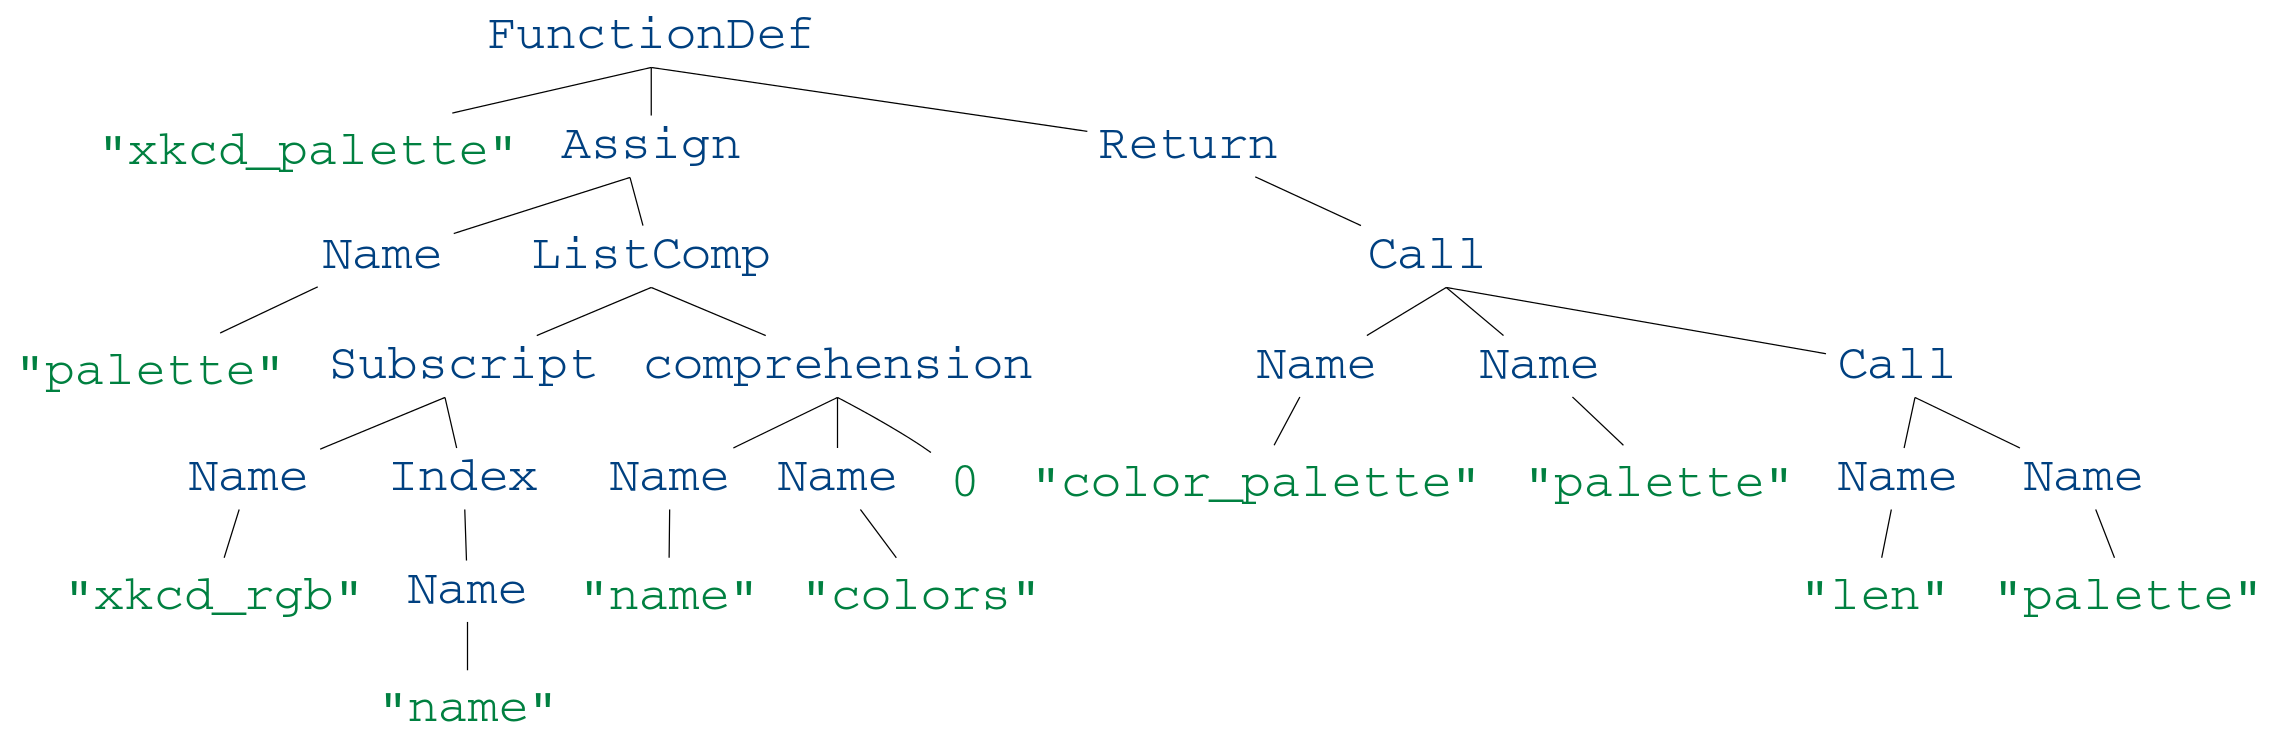
\includegraphics[width=0.8\linewidth]{ImagesCodeRelated/xkcd_palette_strip.png}
\begin{minted}[]{python}
def xkcd_palette(colors):
    palette = [xkcd_rgb[name] for name in colors]
    return color_palette(palette, len(palette))

\end{minted}
\begin{tabular}{l}
\textbf{I}: \mintinline[]{python}{colors}\\
\textbf{D}: list of keys in the `` seaborn.xkcd\_rgb `` dictionary .\\
\textbf{P}: a list of data to read . if none , all other the first will be returned .\\
\end{tabular}

\caption{Code \& List}
\end{listing}

\begin{figure}
\begin{center}
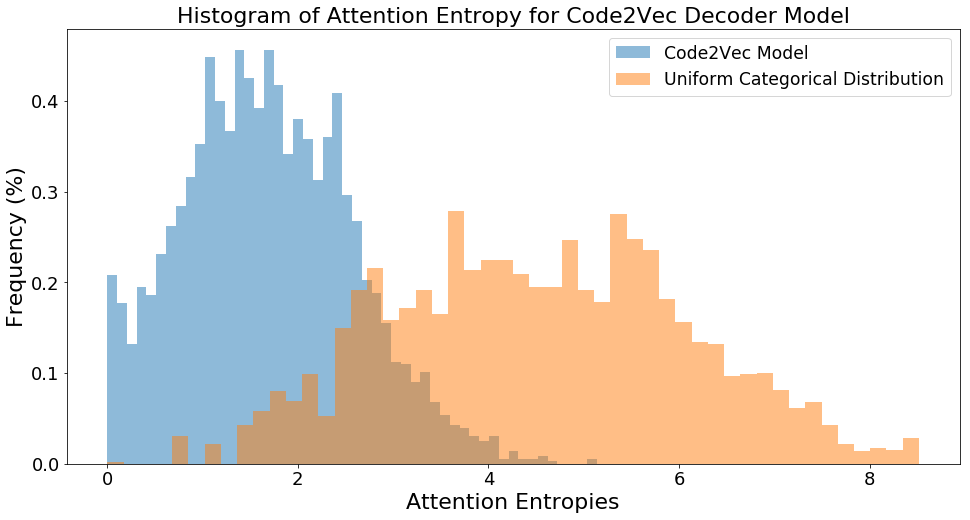
\includegraphics[width=.8\linewidth]{ImagesCodeRelated/code2vec_entropies.png}
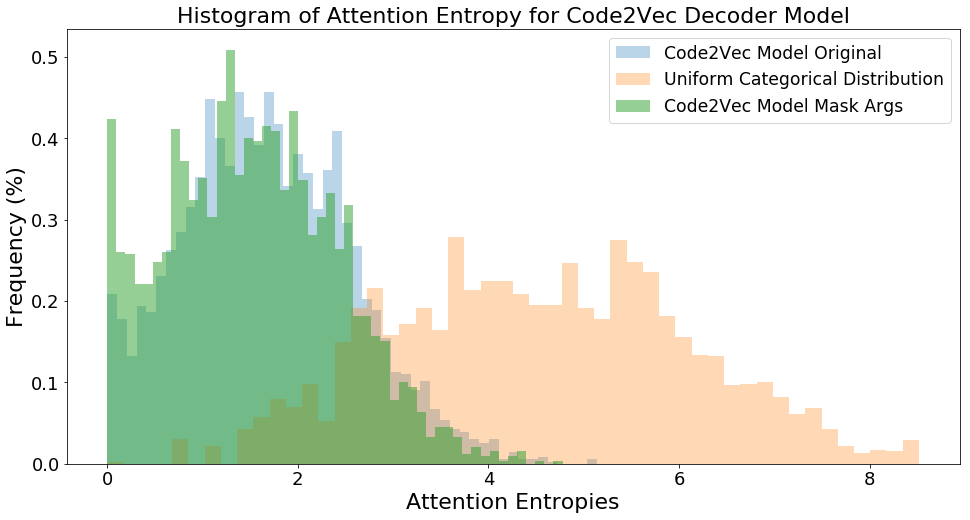
\includegraphics[width=0.6\linewidth]{ImagesCodeRelated/entropies_mask_args.png} 
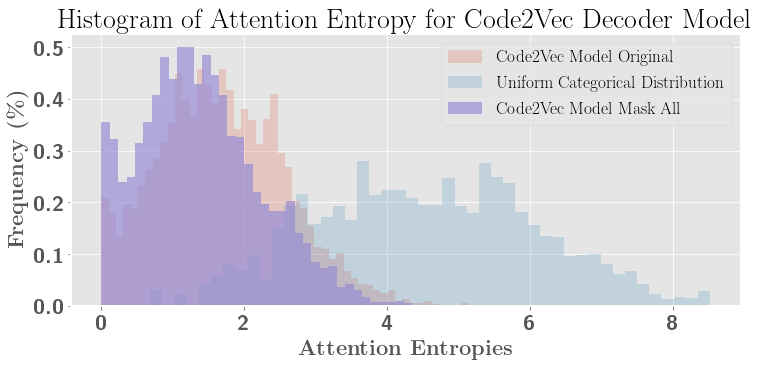
\includegraphics[width=0.6\linewidth]{ImagesCodeRelated/entropies_mask_all.png}
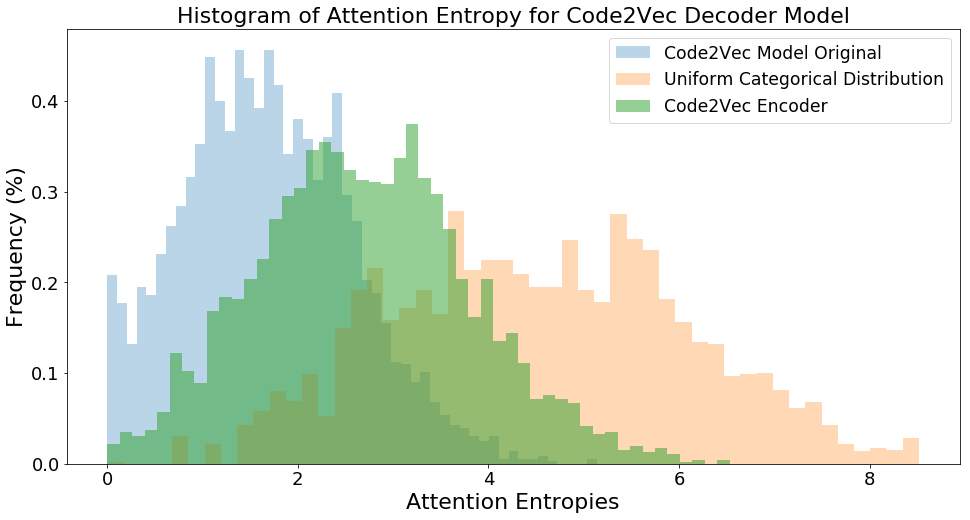
\includegraphics[width=.8\linewidth]{ImagesCodeRelated/save_c2e_encoder.png}
\end{center}
\end{figure}


\begin{enumerate}
    \item With the code lstm we see some of the behaviour we like, but also, only overfitting. There is no sequence so in some cases, a path or a single variable can be informative, but it performs well.
    \item See a single example and distribution of attention.
    \item CLearly there are a lot of spikes compared to uniform. More masking the more spiking, though this is partly due to best bleu. Compare at cross entropy time?
    \item Then look at, bleu per sentence, maybe av bleu per sentence per attn entropy.
    \item Big COMPARE vs ROTE LEARNER - can we conclude this is worth more researcg?
    \item Cna show how choices change w model for given example??

    \item C2VEnc: does combining add anythin? More capacity, check weights.
\end{enumerate}



